\documentclass[aspectratio=169]{beamer}
\usepackage{color,amsmath}
\usepackage{subfigure}
\usepackage{booktabs}
\usepackage{framed}
\usepackage{comment}

\def\vf{\vfill}

%%%%%%%%%%%%%%%%%%%%%%%%%%
\title[]{Zero variable cost experiments and MusicLab}
\author[]{Matthew J. Salganik\\Department of Sociology\\Princeton University}
\date[]{Summer Institutes in Computational Social Science\\June 22, 2019
\vfill
\begin{flushleft}
{\scriptsize
The Summer Institutes in Computational Social Science is supported by grants from the Russell Sage Foundation and the Alfred P. Sloan Foundation.}
\end{flushleft}
\begin{flushright}

\includegraphics[width=0.1\textwidth]{figures/cc-by.png}
\end{flushright}
}
\begin{document}
%%%%%%%%%%%%%%%%%%%%%%%%%%
\frame{\titlepage}
%%%%%%%%%%%%%%%%%%%%%%%%%%
\begin{frame}

{\Large
\begin{center}
Experiments at scale
\end{center}
}
\end{frame}
%%%%%%%%%%%%%%%%%%%%%%%%%
\begin{frame}

\begin{center}
\only<1>{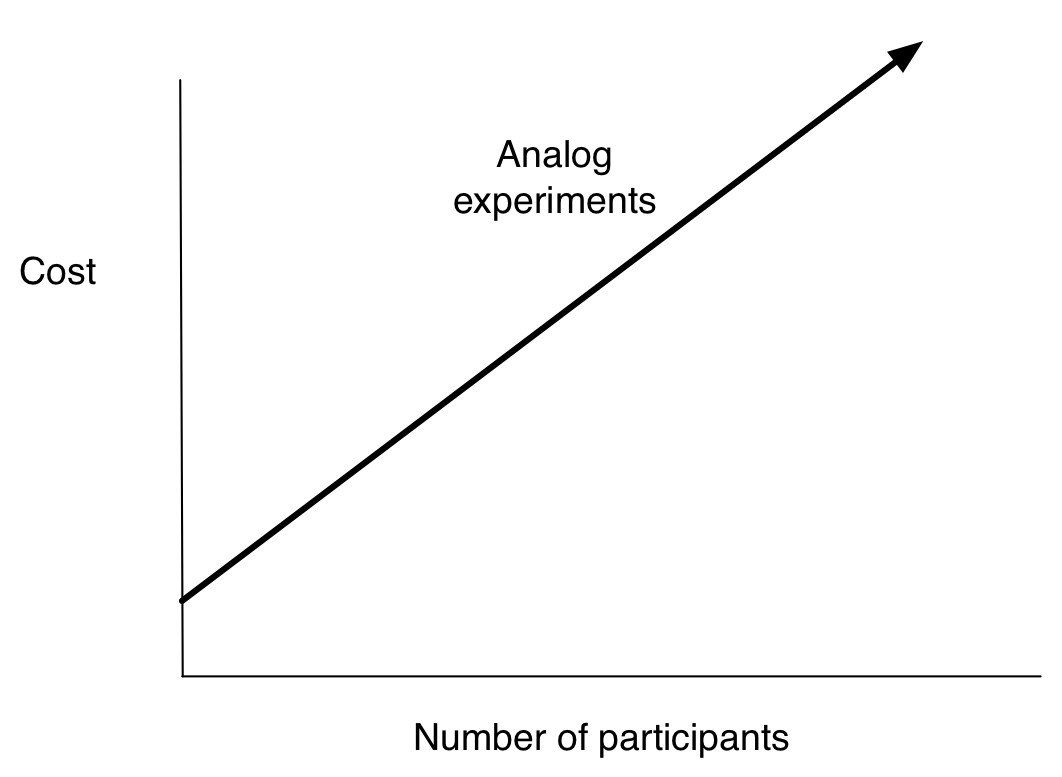
\includegraphics[width=0.8\textwidth]{figures/zero_variable_cost_experiments_analog}}
\only<2>{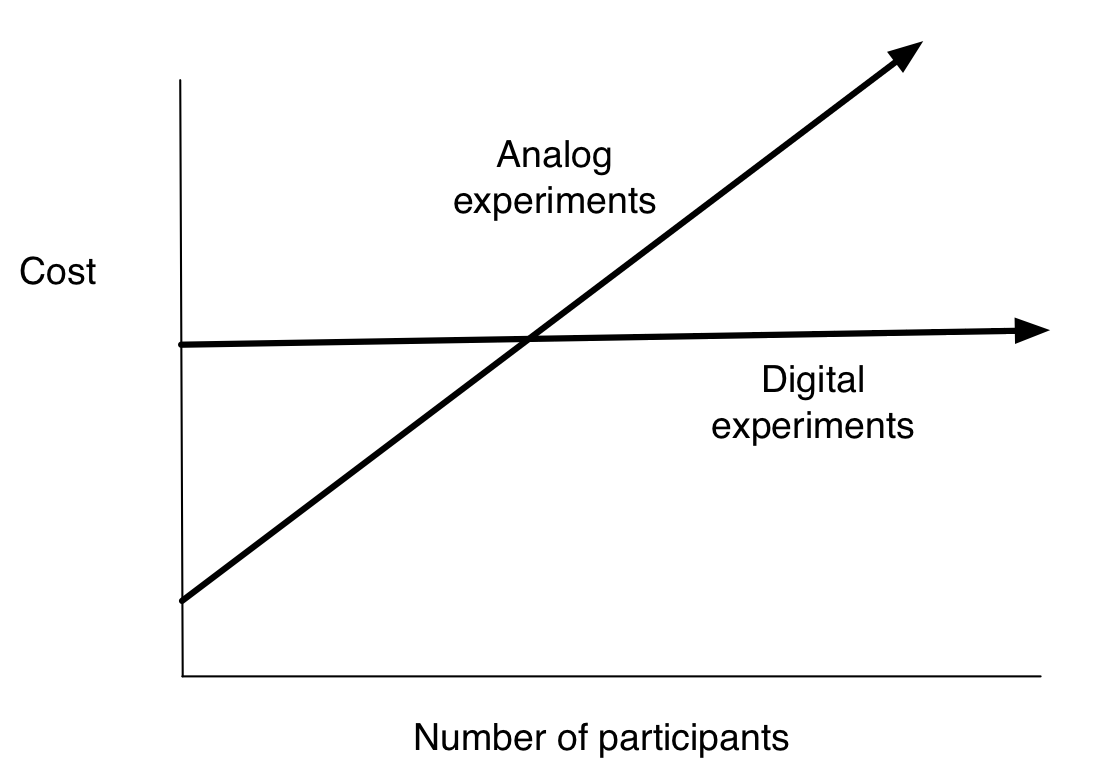
\includegraphics[width=0.8\textwidth]{figures/zero_variable_cost_experiments_both}}
\end{center}

\end{frame}
%%%%%%%%%%%%%%%%%%%%%%%%%
\begin{frame}

Main sources of variable costs:
\begin{itemize}
\item staff time
\item participant payment
\end{itemize}

\vf
\pause
Solutions:
\begin{itemize}
\item Automation (your experiments should run while you sleep)
\item Design enjoyable experiments
\end{itemize}

\end{frame}
%%%%%%%%%%%%%%%%%%%%%%%%
\begin{frame}

\begin{figure}
  \centering
  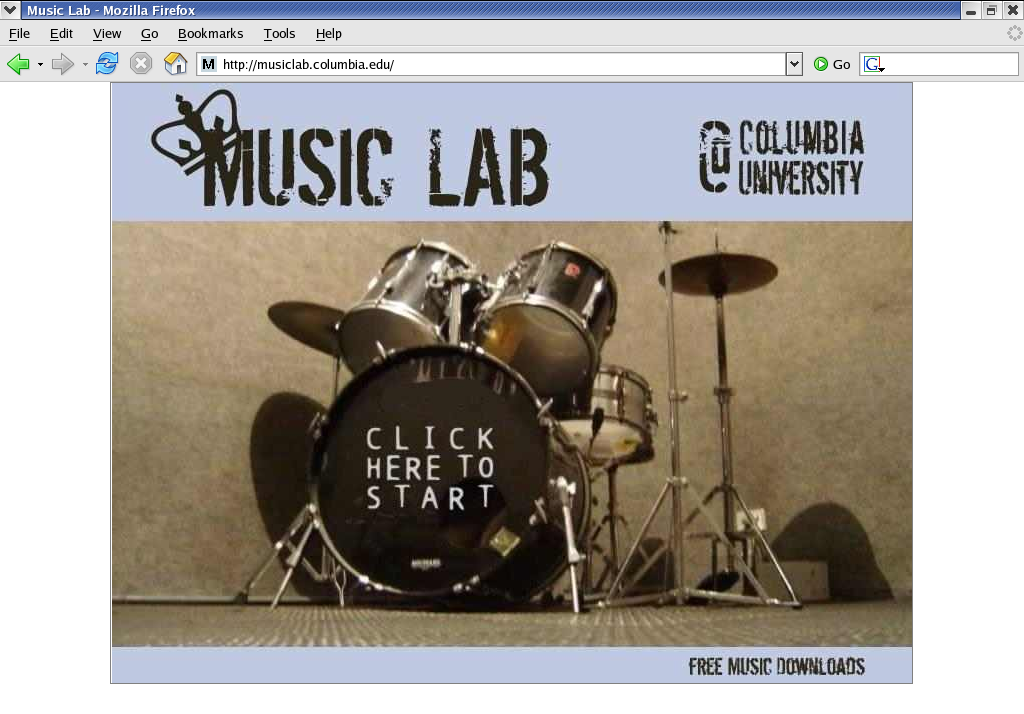
\includegraphics[width = 0.9\textwidth]{figures/splashscreen}
\end{figure}

Music Lab: a zero variable cost experiment with Peter Dodds and Duncan Watts

\end{frame}
%%%%%%%%%%%%%%%%%%%%%%%%%%%%%%%%%
\begin{frame}

\begin{figure}
  \centering
  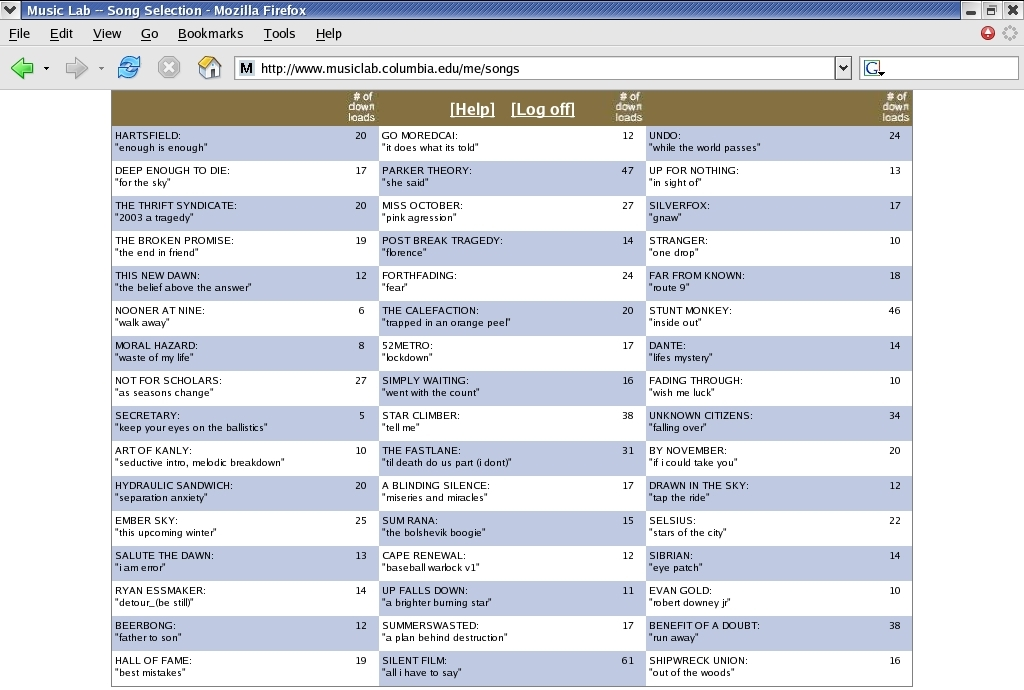
\includegraphics[width = 0.9\textwidth]{figures/info-v1-cut}
\end{figure}

\end{frame}
%%%%%%%%%%%%%%%%%%%%%%%%%%%%%%%%%
\begin{frame} 

\begin{figure}
  \centering
  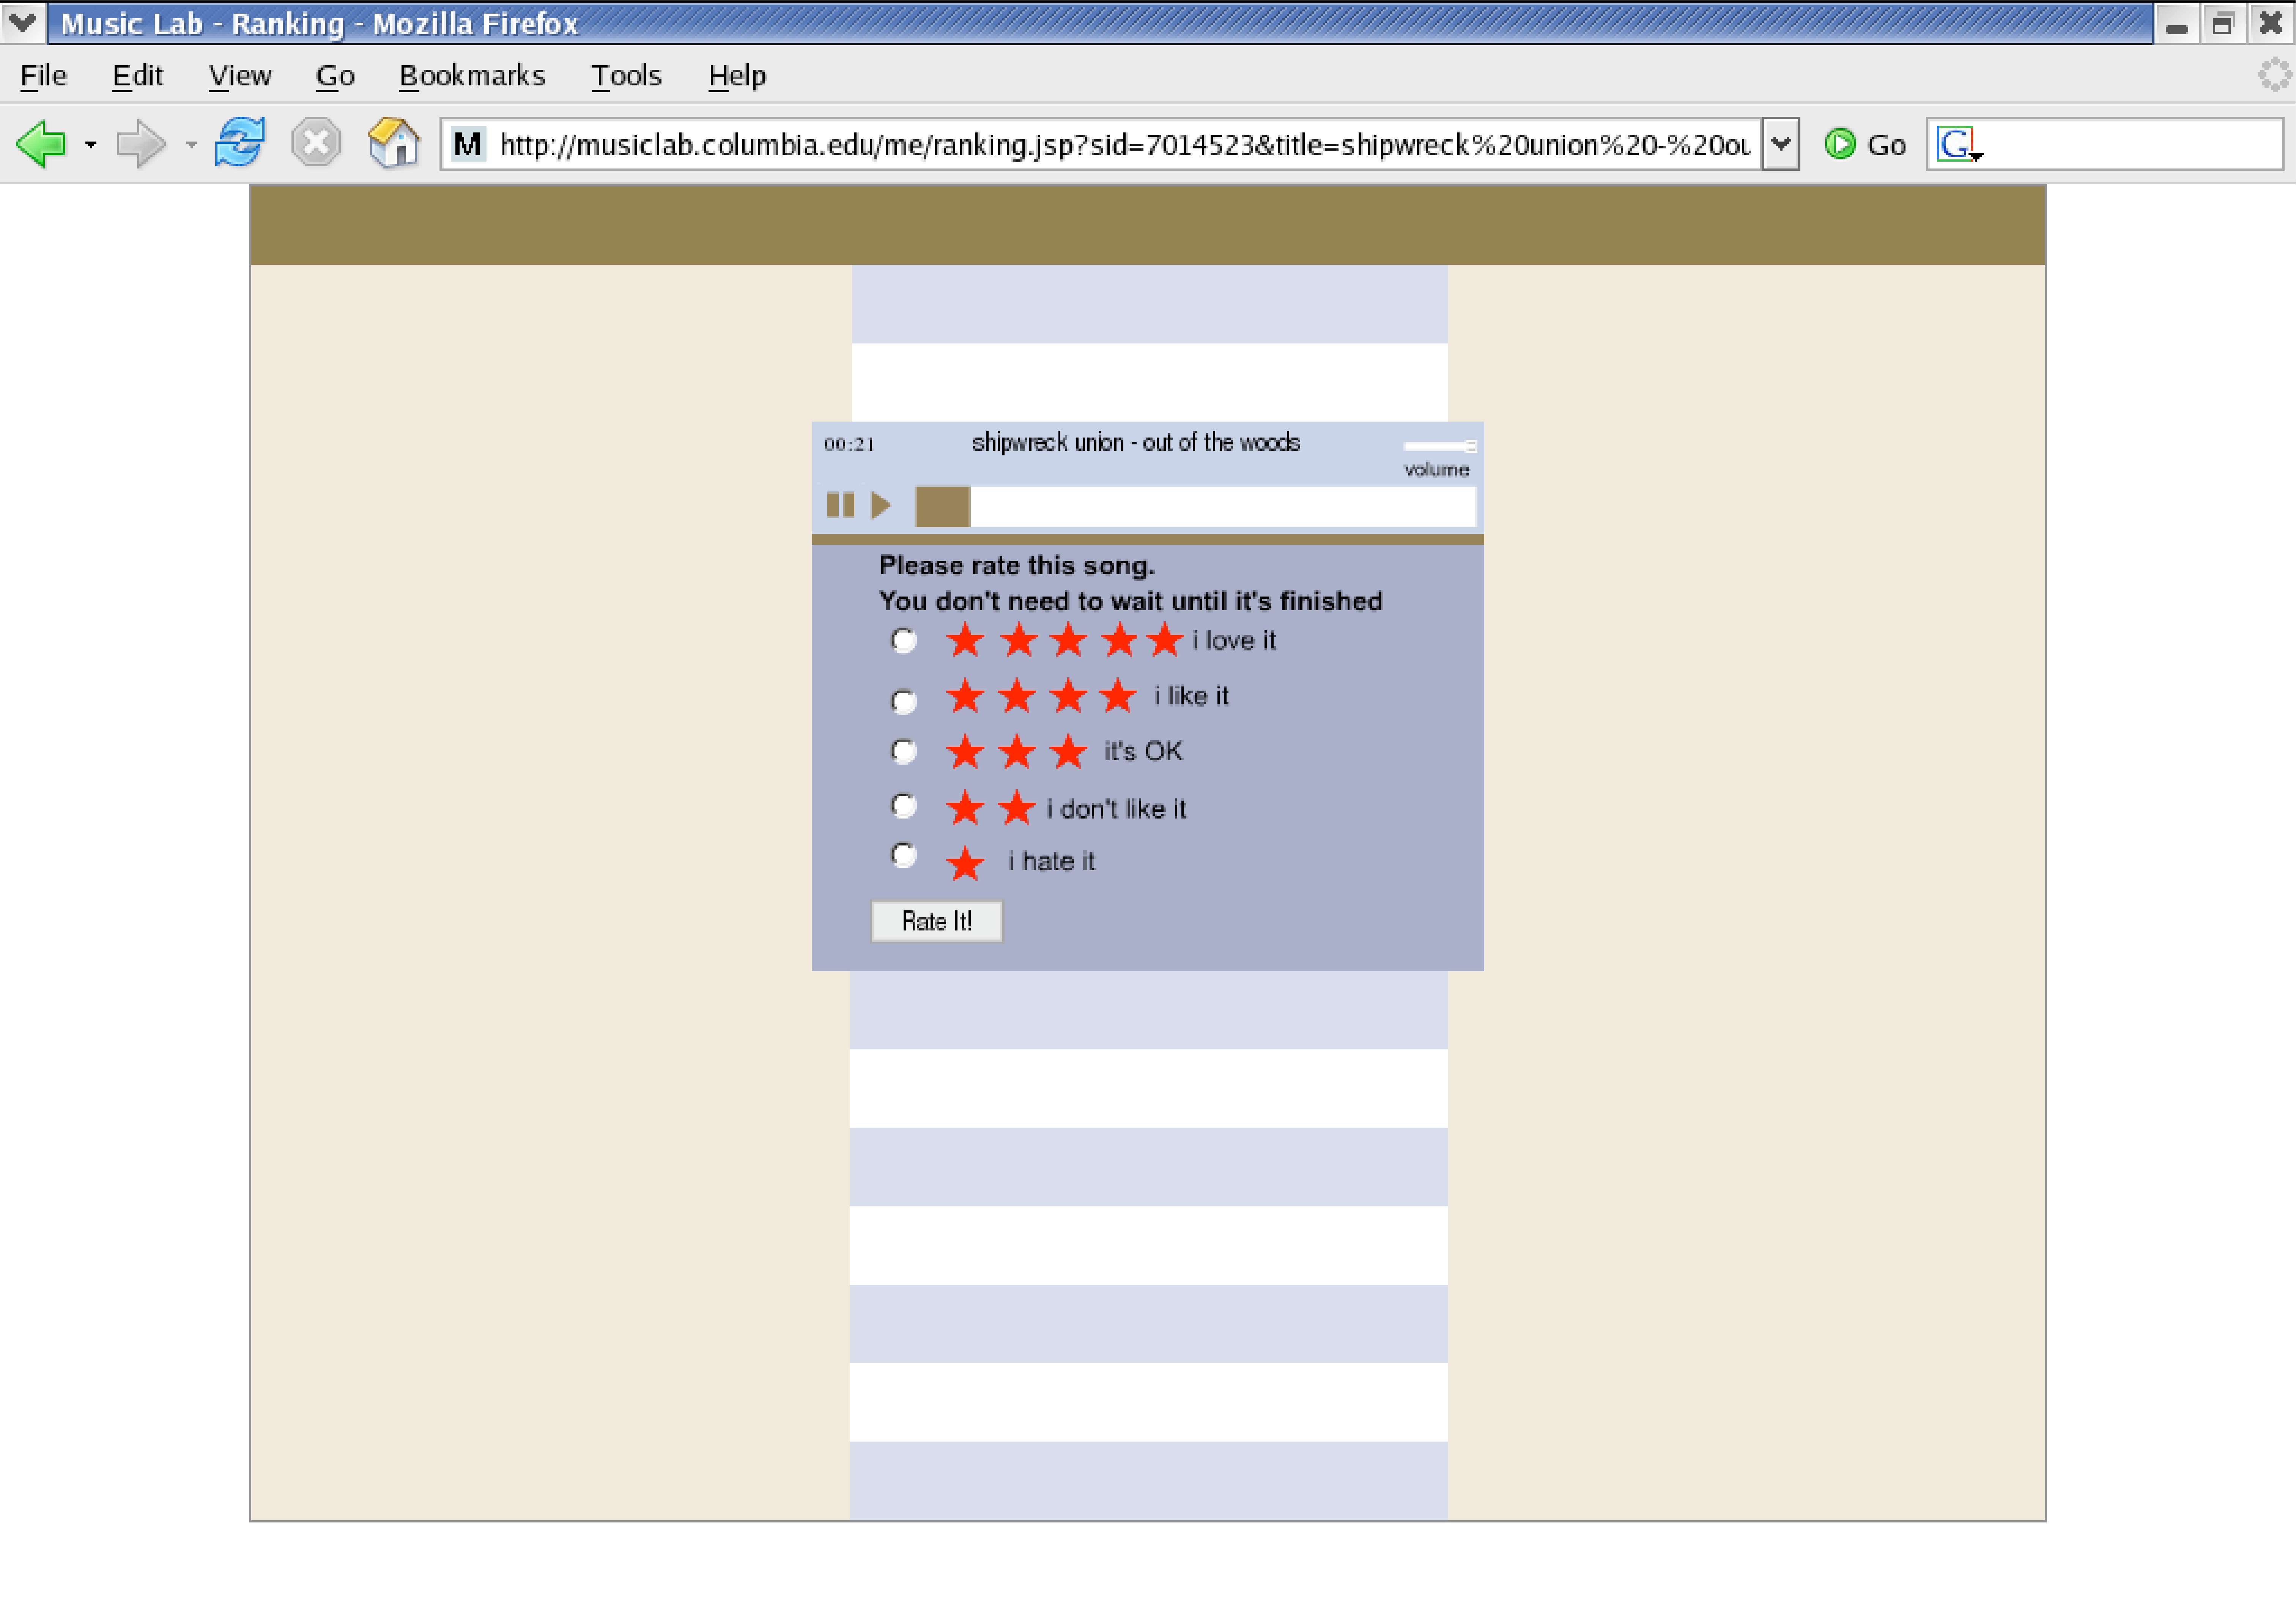
\includegraphics[width = 0.9\textwidth]{figures/listenscreen}
\end{figure}

\end{frame}
%%%%%%%%%%%%%%%%%%%%%%%%%%%%%%%%%
\begin{frame}

\begin{figure}
  \centering
  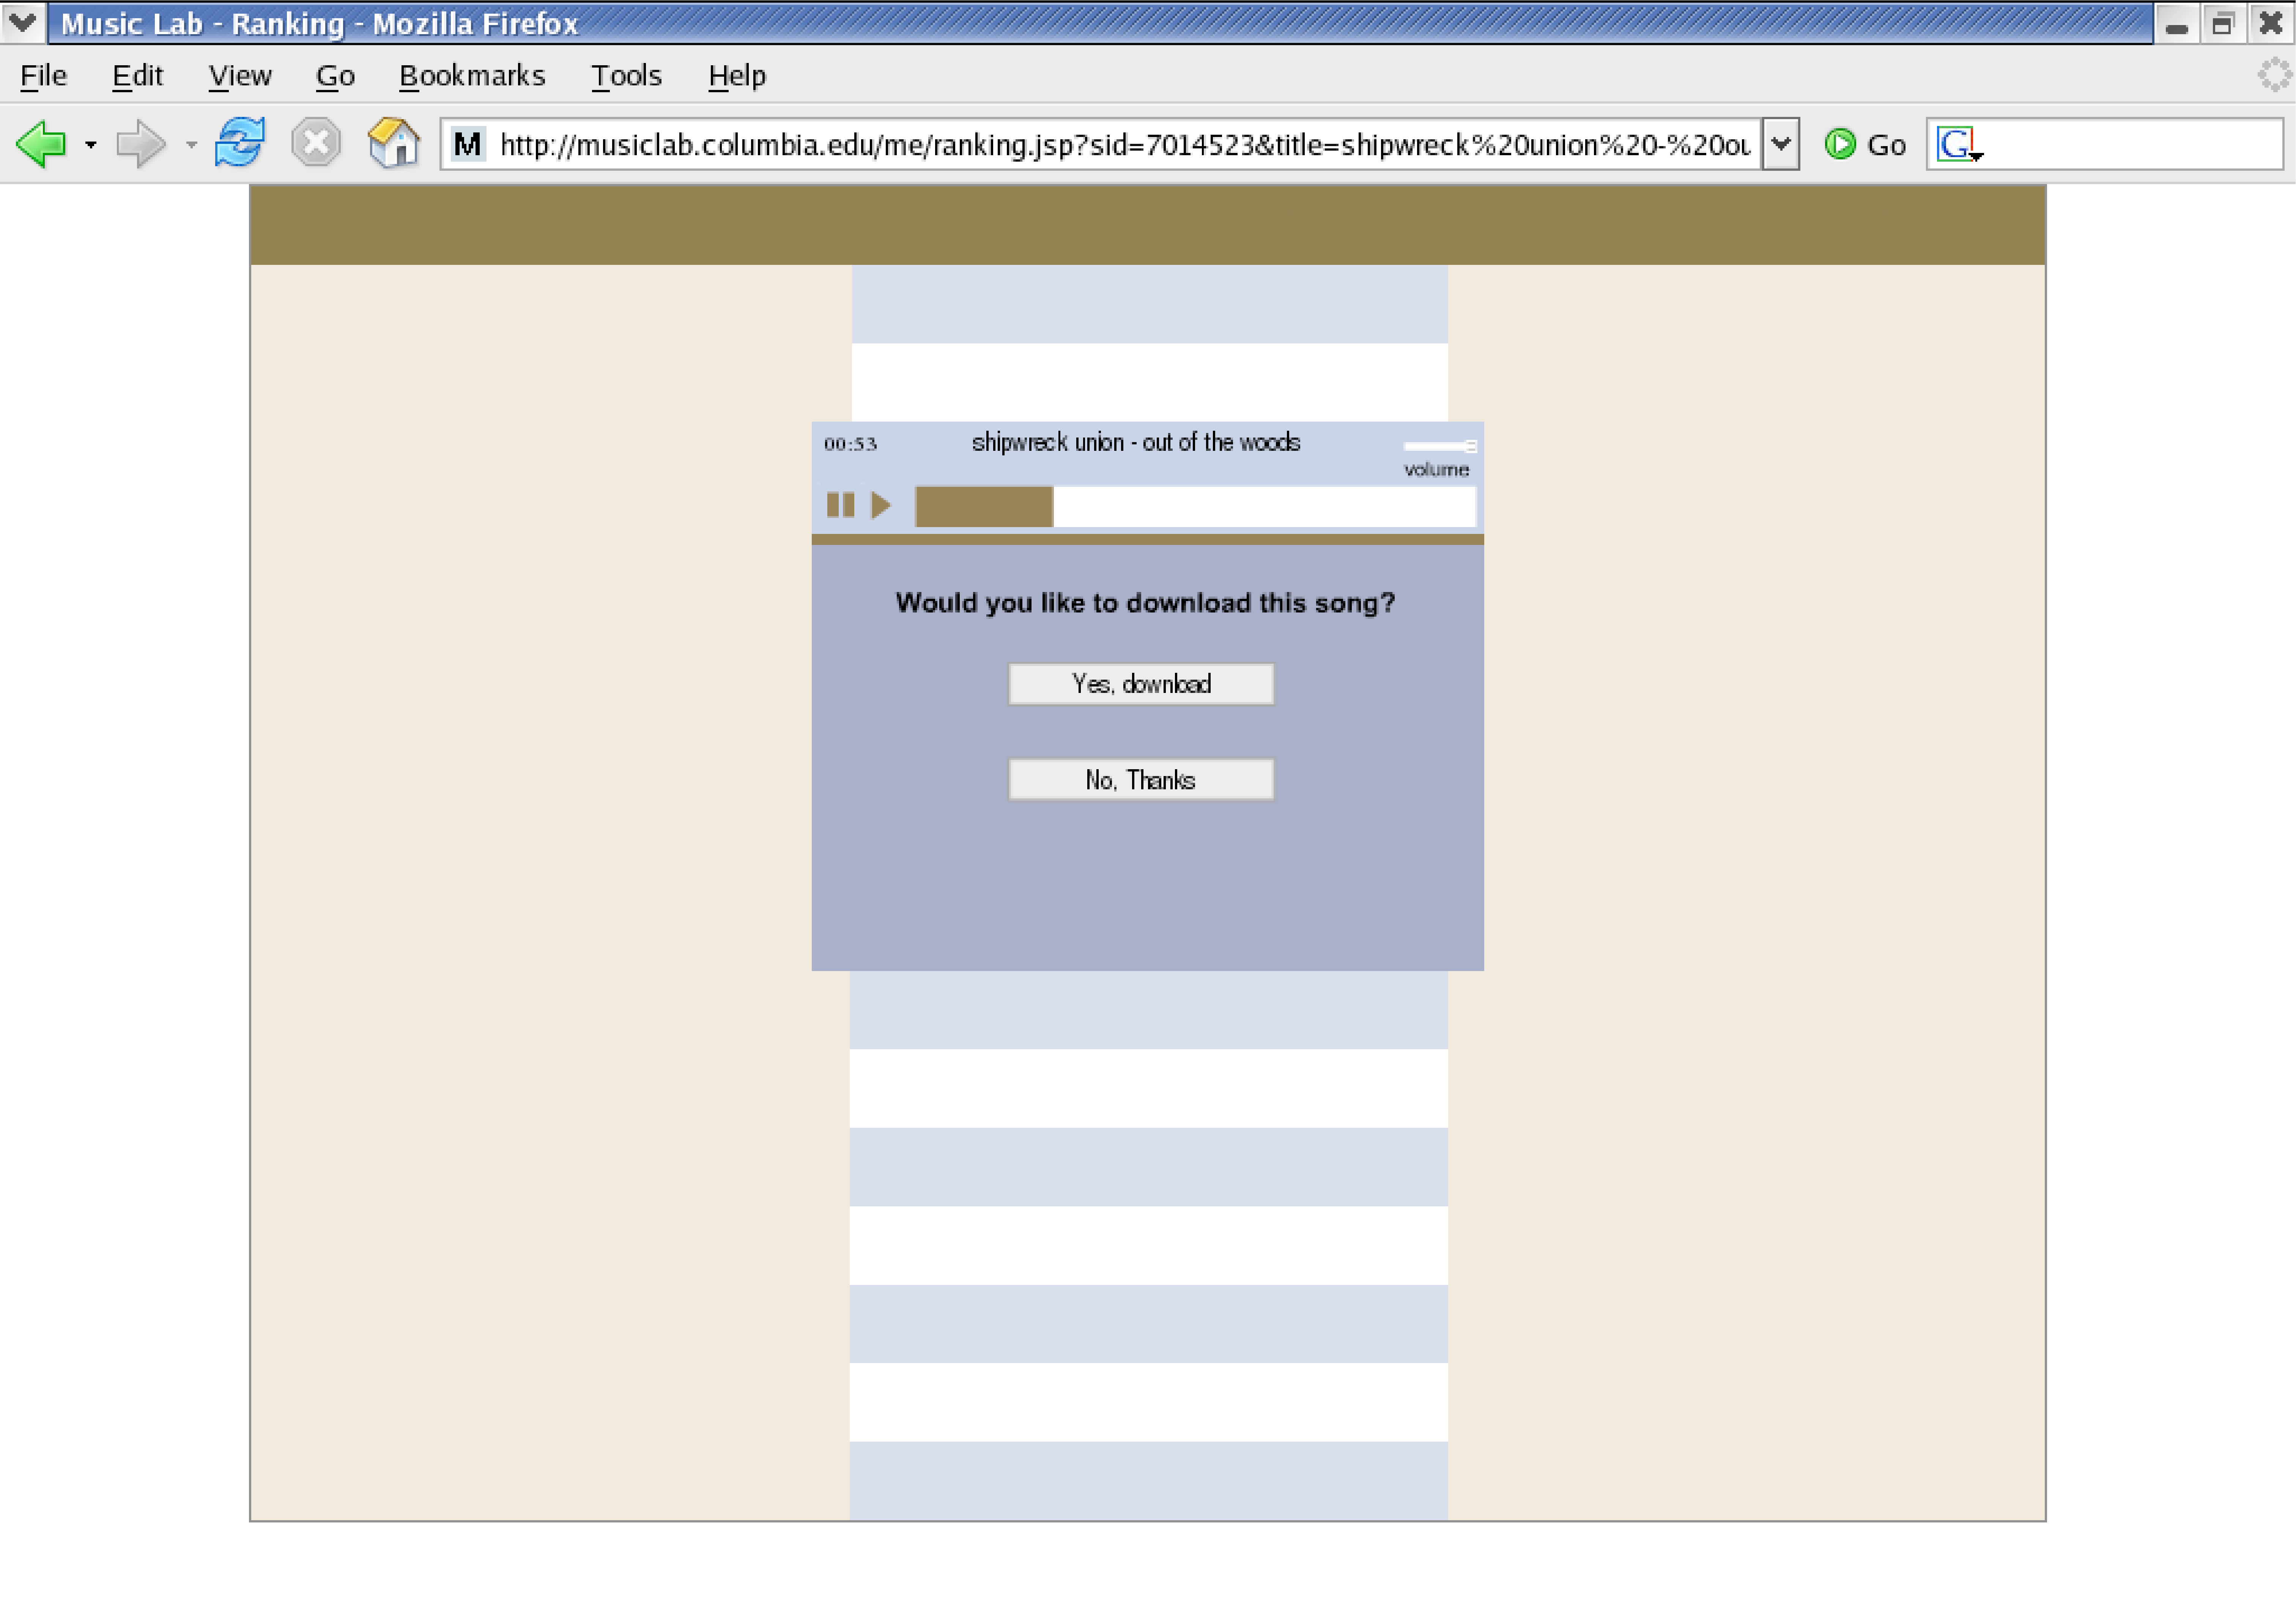
\includegraphics[width = 0.9\textwidth]{figures/downloadscreen}
\end{figure}

\end{frame}
%%%%%%%%%%%%%%%%%%%%%%%%%%%%%%%%%%
\begin{frame}

\begin{figure}
  \centering
  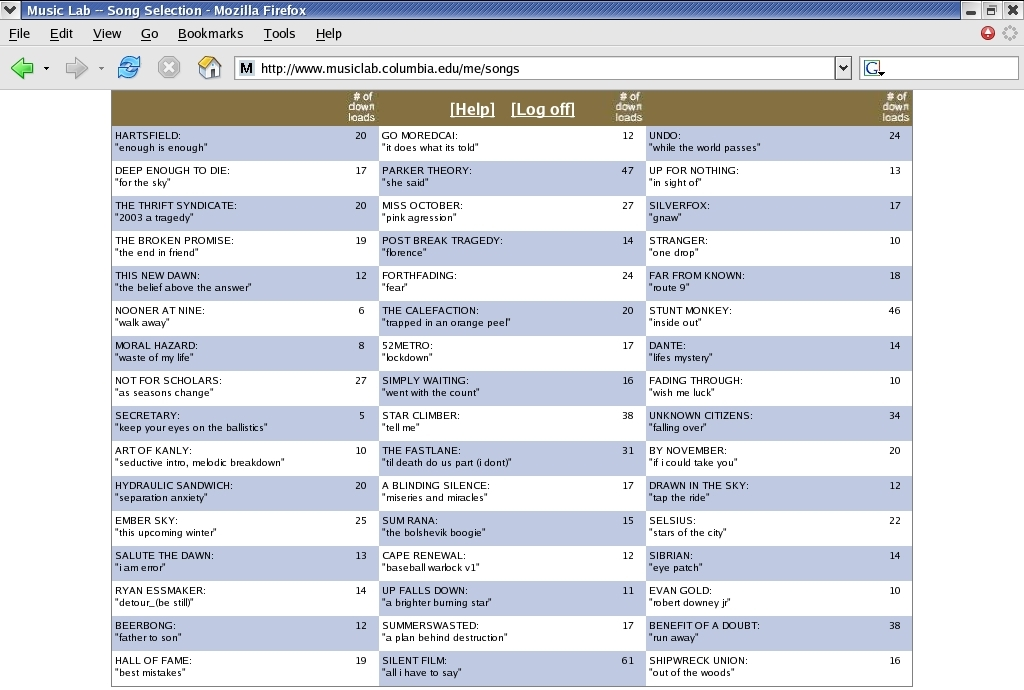
\includegraphics[width = 0.9\textwidth]{figures/info-v1-cut}
\end{figure}

\end{frame}
%%%%%%%%%%%%%%%%%%%%%%%%%%%%%%%%%
\begin{frame}

\begin{figure}
  \centering
  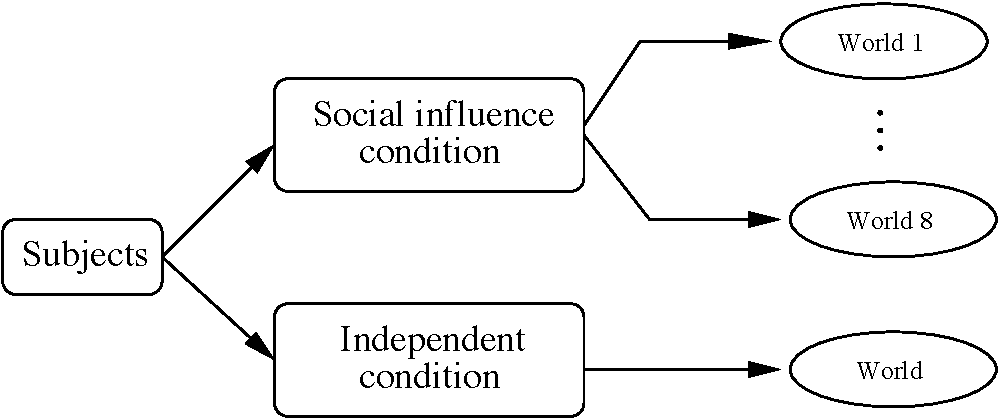
\includegraphics[width=0.9\textwidth]{figures/expdesign_4}
\end{figure}

\end{frame}
%%%%%%%%%%%%%%%%%%%%%%%%%%%%%%%%%%
\begin{frame}

\setcounter{subfigure}{0}
\begin{figure}
  \centering
     \subfigure[Less social influence]{
     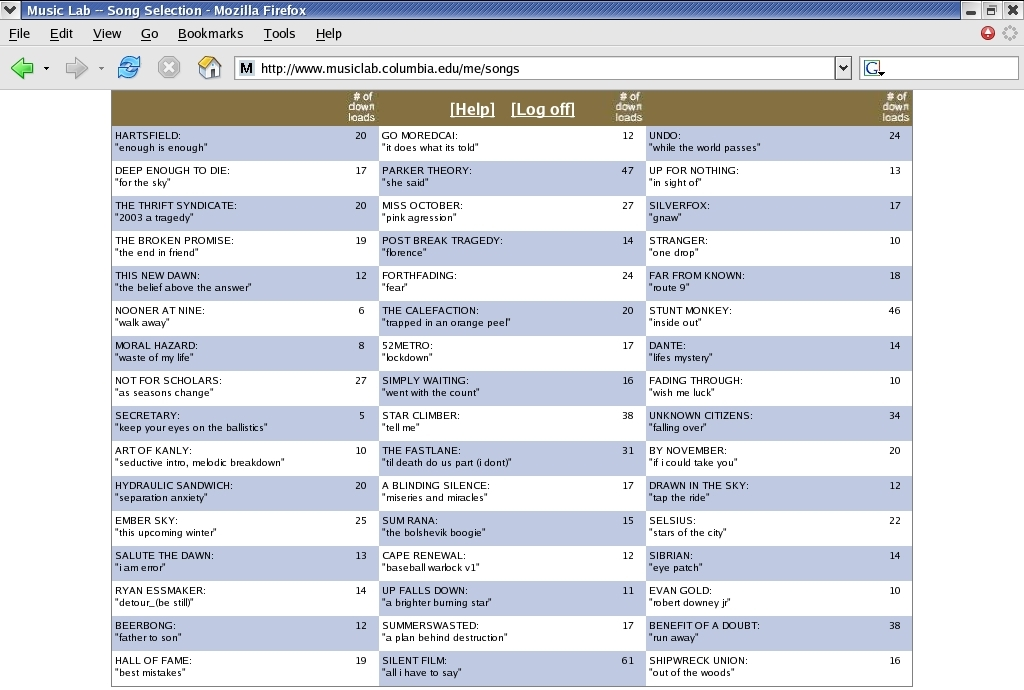
\includegraphics[width=0.45\textwidth]{figures/info-v1-cut}}
  \hspace{0in}
     \subfigure[More social influence]{
     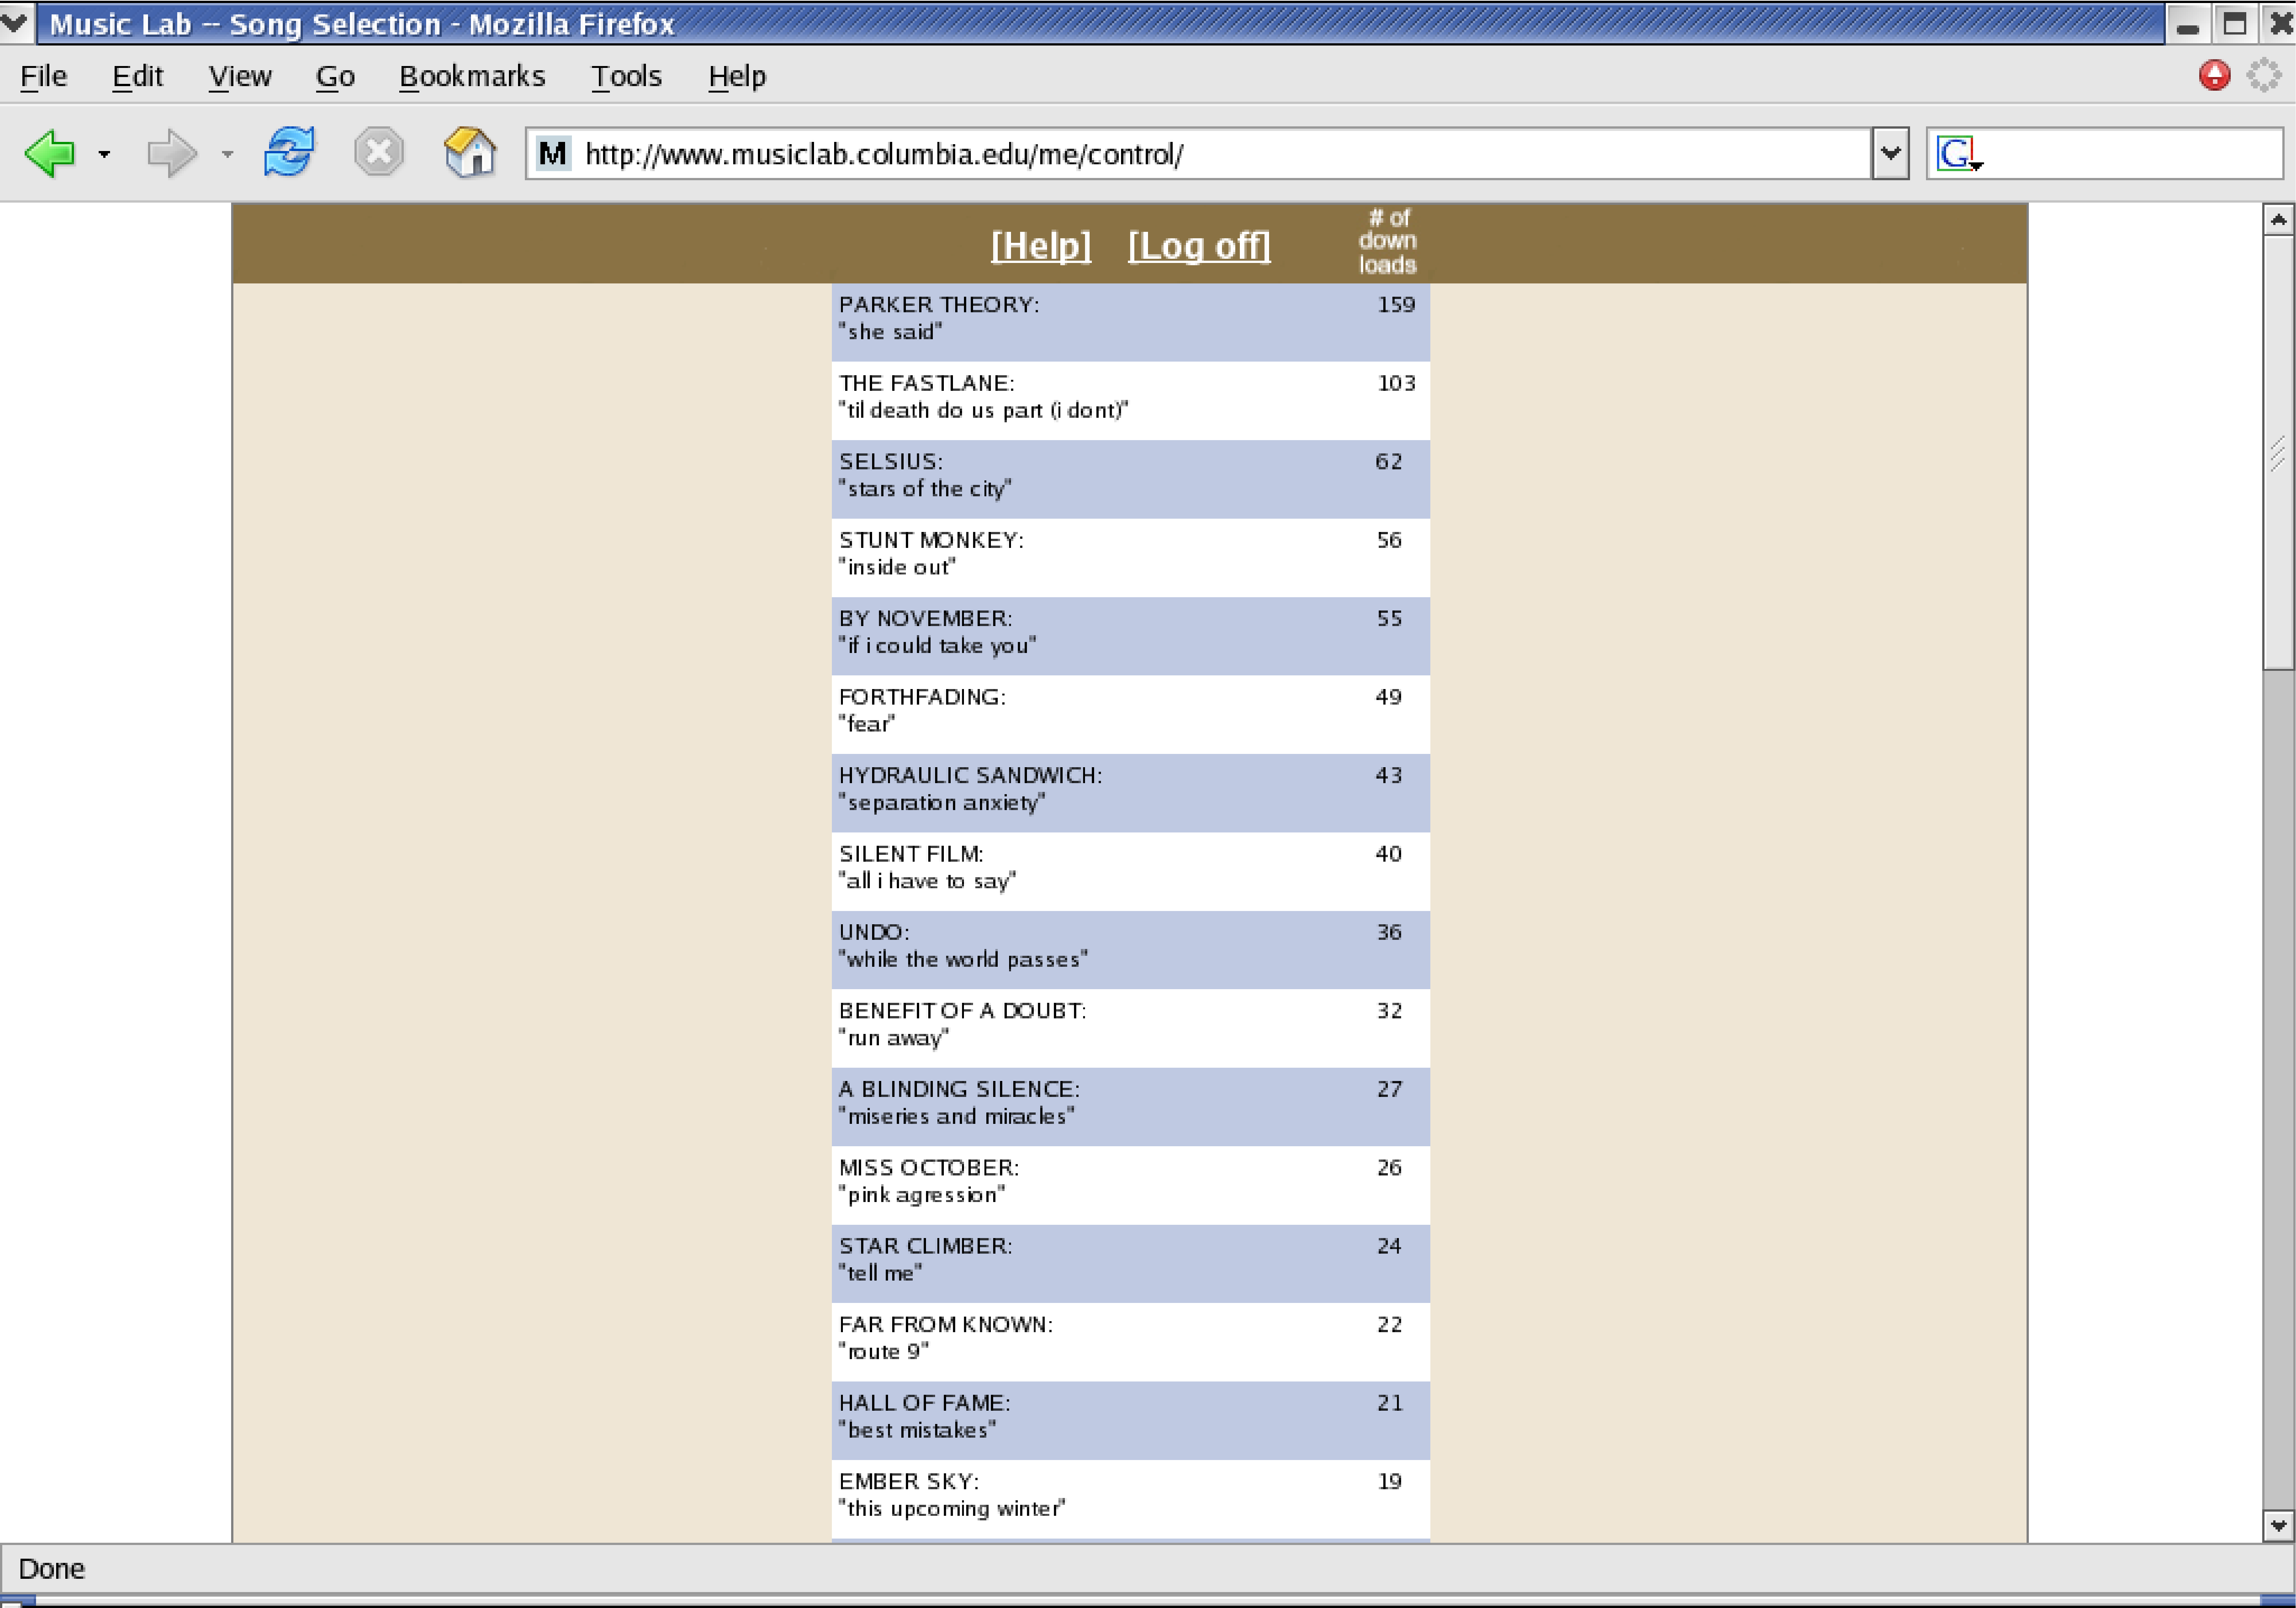
\includegraphics[width=0.45\textwidth]{figures/info-v2-original}}
\end{figure}

\end{frame}
%%%%%%%%%%%%%%%%%%%%%%%%%%%%%%%%%%
\begin{frame}

\begin{figure}
  \centering
   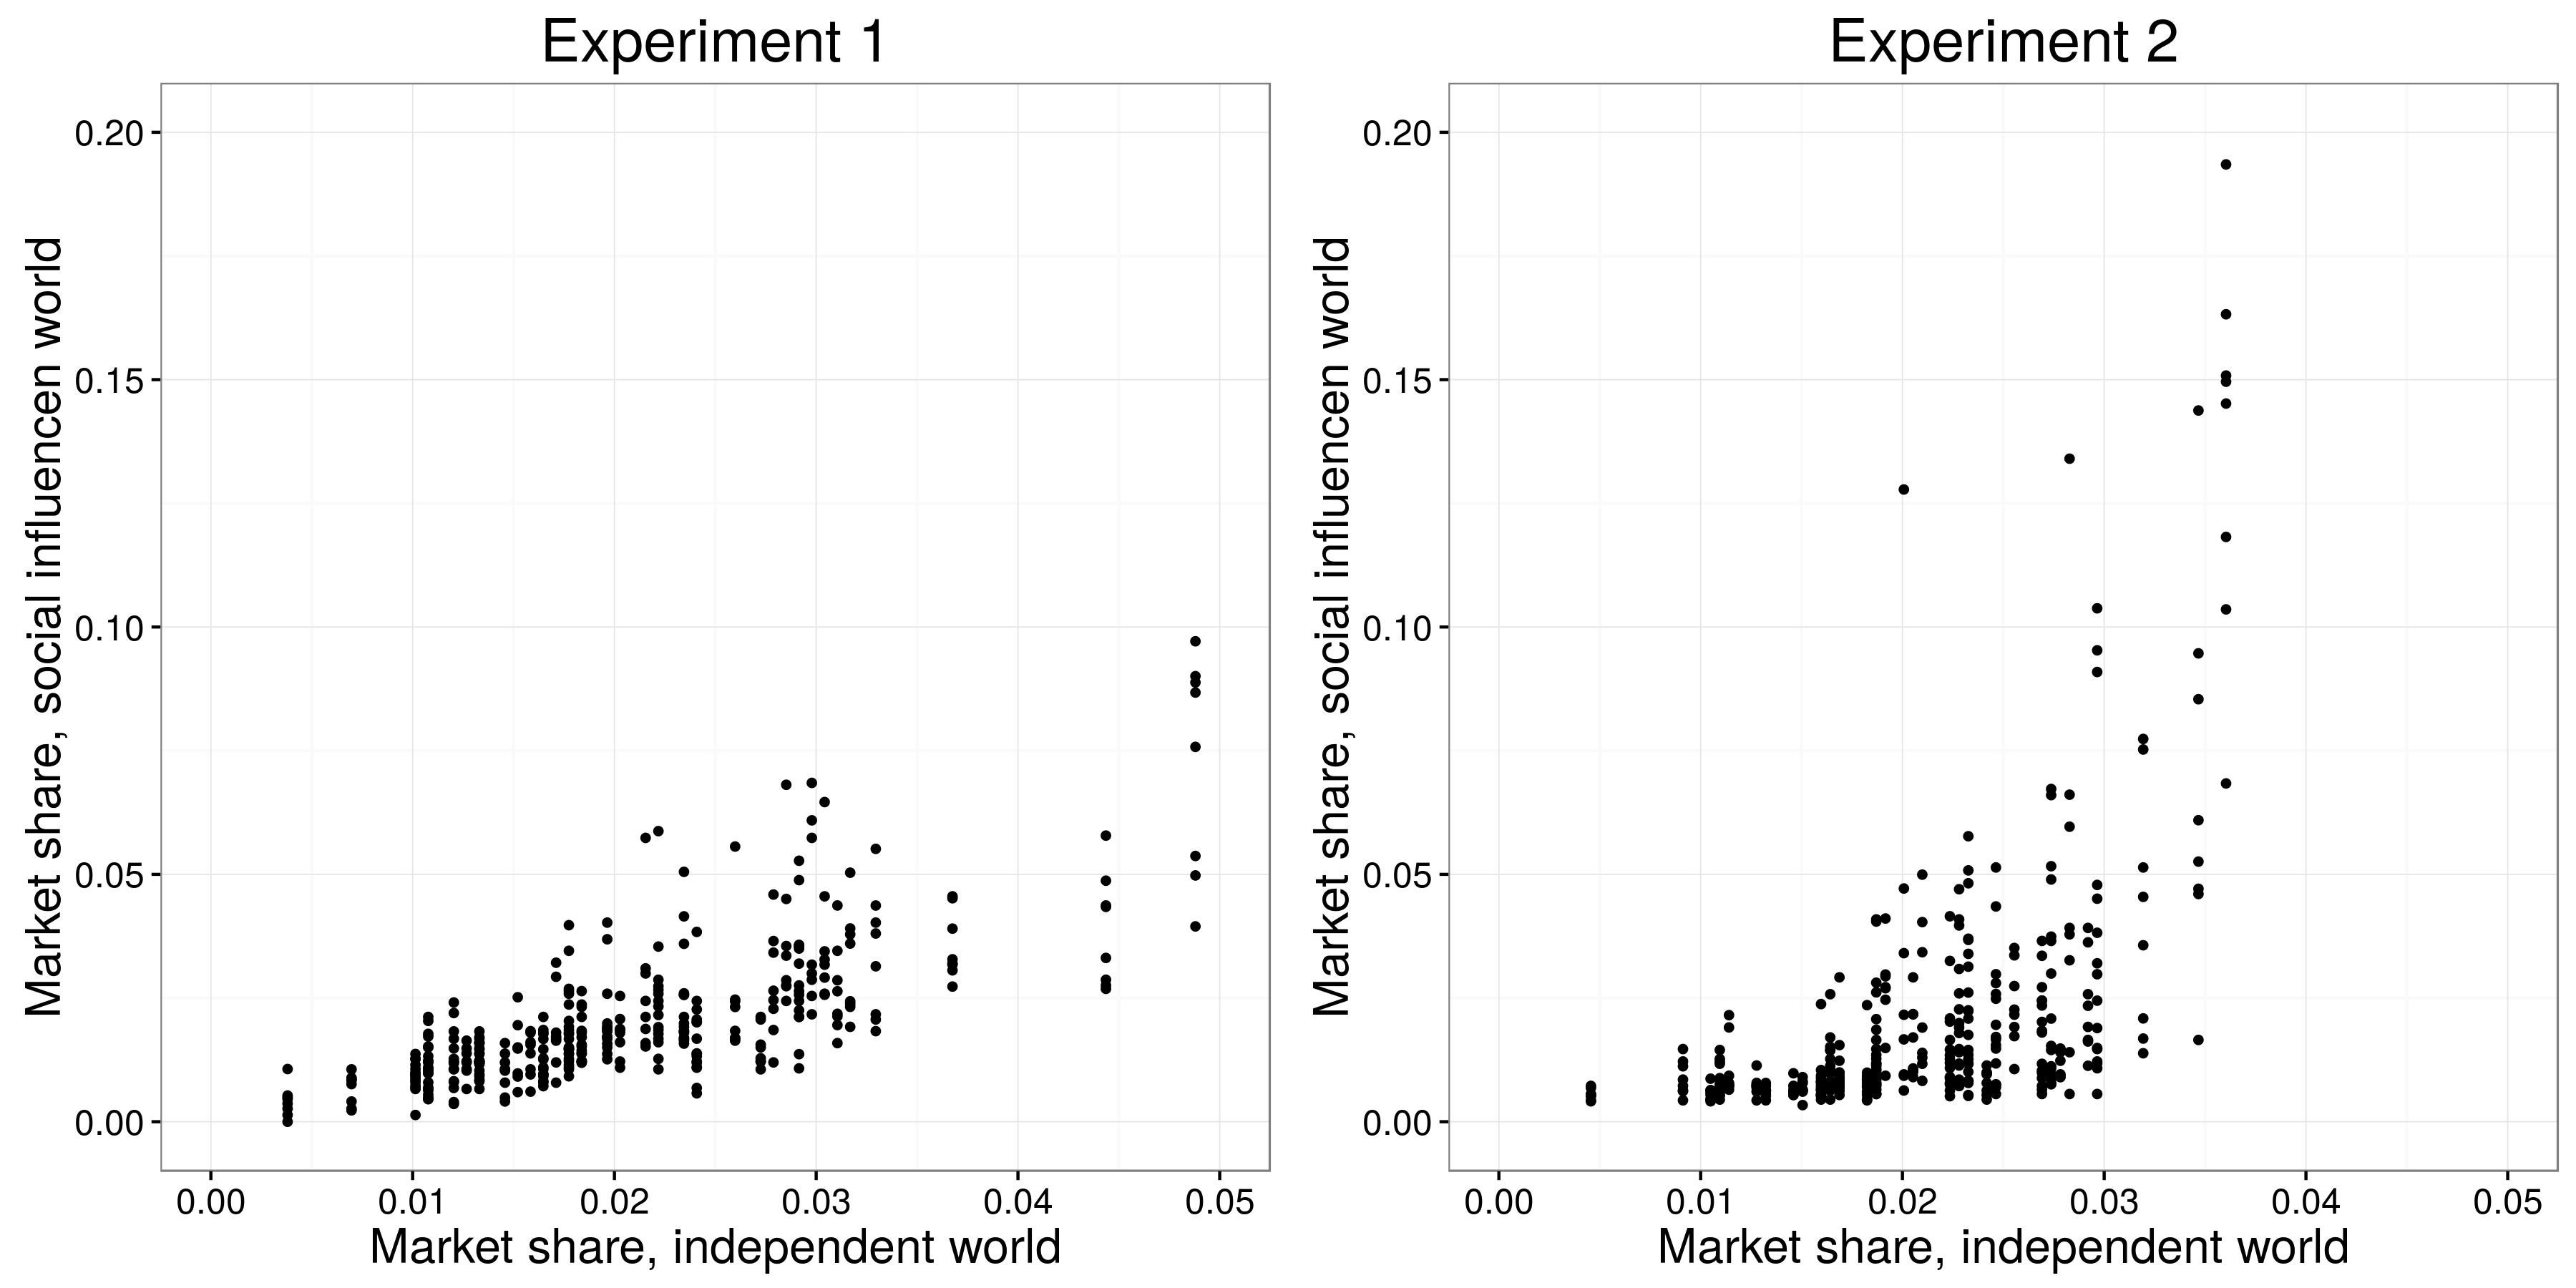
\includegraphics[width=0.95\textwidth]{figures/bitbybit4-23_salganik_experimental_2006_fig3ac}
\end{figure}

Results: \pause
\begin{itemize}
\item More social influence leads to more unpredictability
\pause
\item You can predict failure but you can't predict success
\end{itemize}
 
\end{frame}
%%%%%%%%%%%%%%%%%%%%%%%%%%%%%%%%%%
\begin{frame}

\begin{figure}
  \centering
  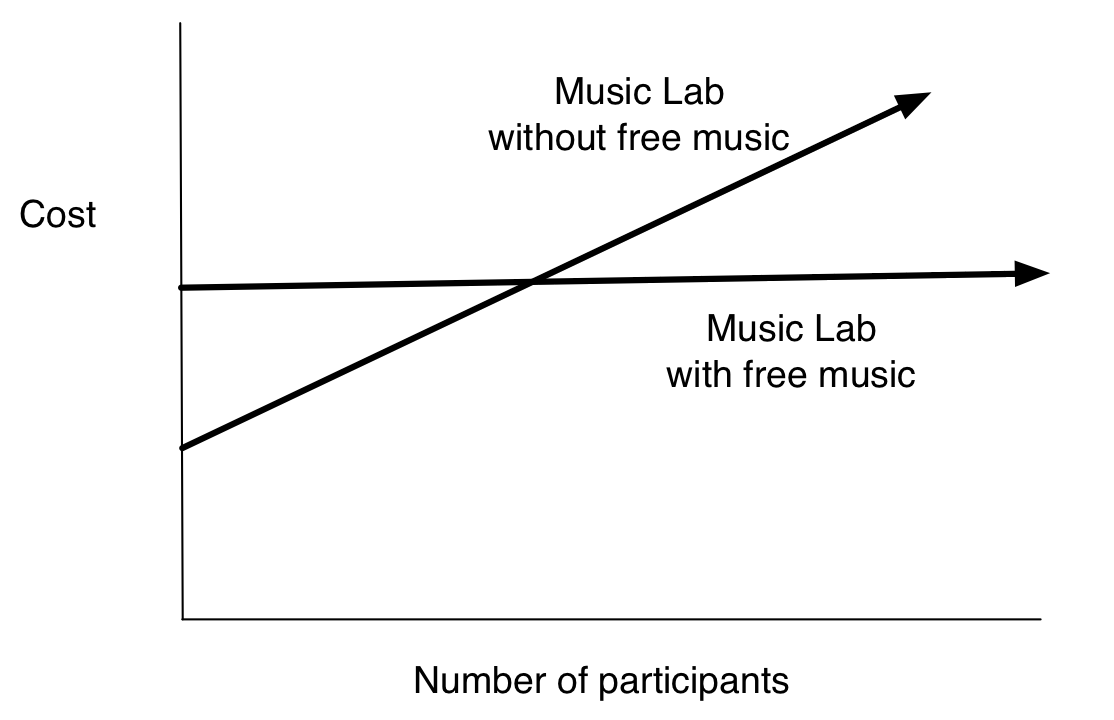
\includegraphics[width=0.7\textwidth]{figures/zero_variable_cost_experiments_musiclab}
\end{figure}

\vf
\pause
\Large{Zero variable cost is a means not an end.}

\end{frame}
%%%%%%%%%%%%%%%%%%%%%%%%
\begin{frame}

{\Large
\begin{center}
Behind the MusicLab?
\end{center}
}

\end{frame}
%%%%%%%%%%%%%%%%%%%%%%%%
\begin{frame}

\begin{figure}
  \centering
  
\includegraphics[width=0.8\textwidth]{figures/milkman_temporal_2012_title.png}
\end{figure}

\vf
\tiny{\url{http://dx.doi.org/10.1177/0956797611434539}}

\end{frame}
%%%%%%%%%%%%%%%%%%%%%%%%
\begin{frame}

{\texttt
Dear Professor Salganik,\\ 

I am writing you because I am a prospective Ph.D. student with considerable interest in your research. My plan is to apply to Ph.D. programs this coming fall, and I am eager to learn as much as I can about research opportunities in the meantime.\\

I will be on campus today, and although I know it is short notice, I was wondering if you might have 10 minutes when you would be willing to meet with me to briefly talk about your work and any possible opportunities for me to get involved in your research. Any time that would be convenient for you would be fine with me, as meeting with you is my first priority during this campus visit.\\

Thank you in advance for your consideration.\\

Sincerely,\\
Carlos Lopez
}

\end{frame}
%%%%%%%%%%%%%%%%%%%%%%%%
\begin{frame}

\begin{figure}
  \centering
  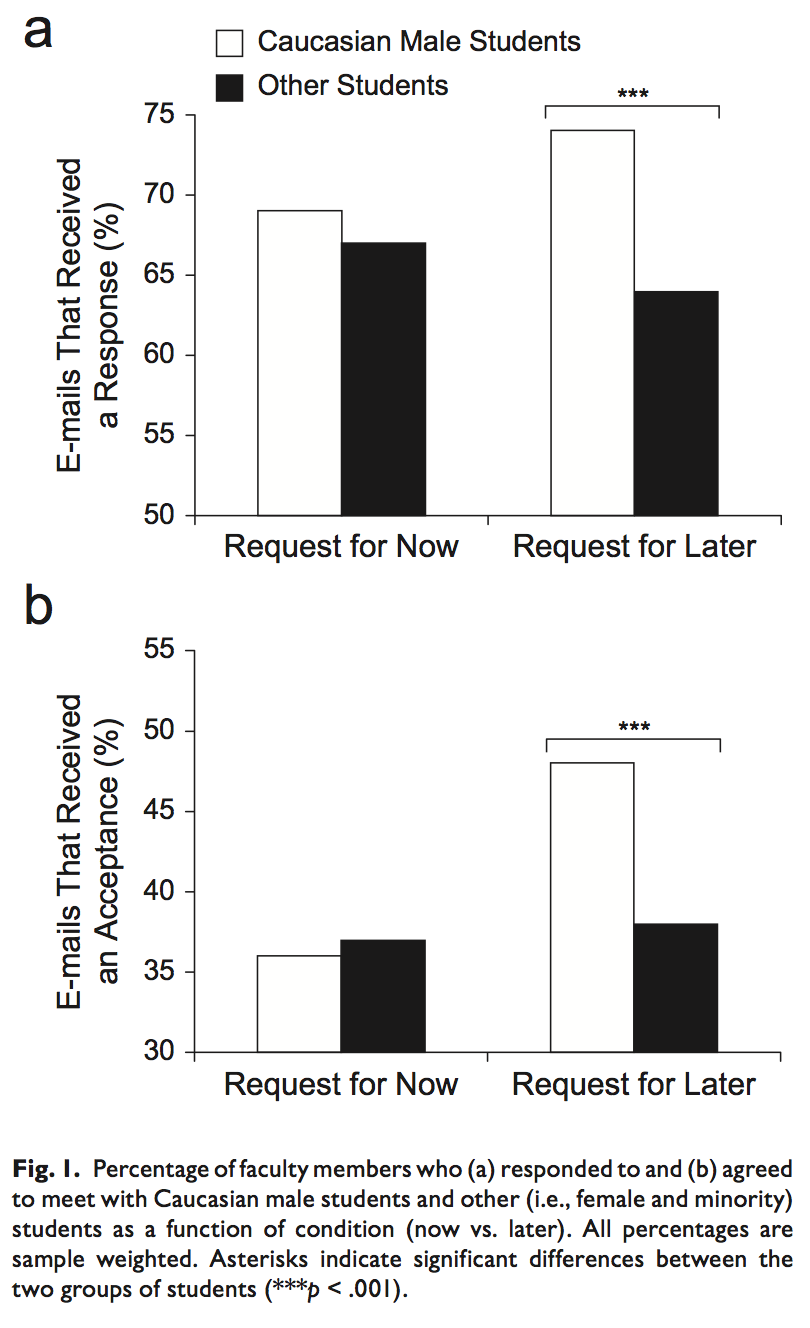
\includegraphics[height=0.8\textheight]{figures/milkman_temporal_2012_fig1.png}
\end{figure}

\end{frame}
%%%%%%%%%%%%%%%%%%%%%%%%
\begin{frame}

\begin{figure}
  \centering
  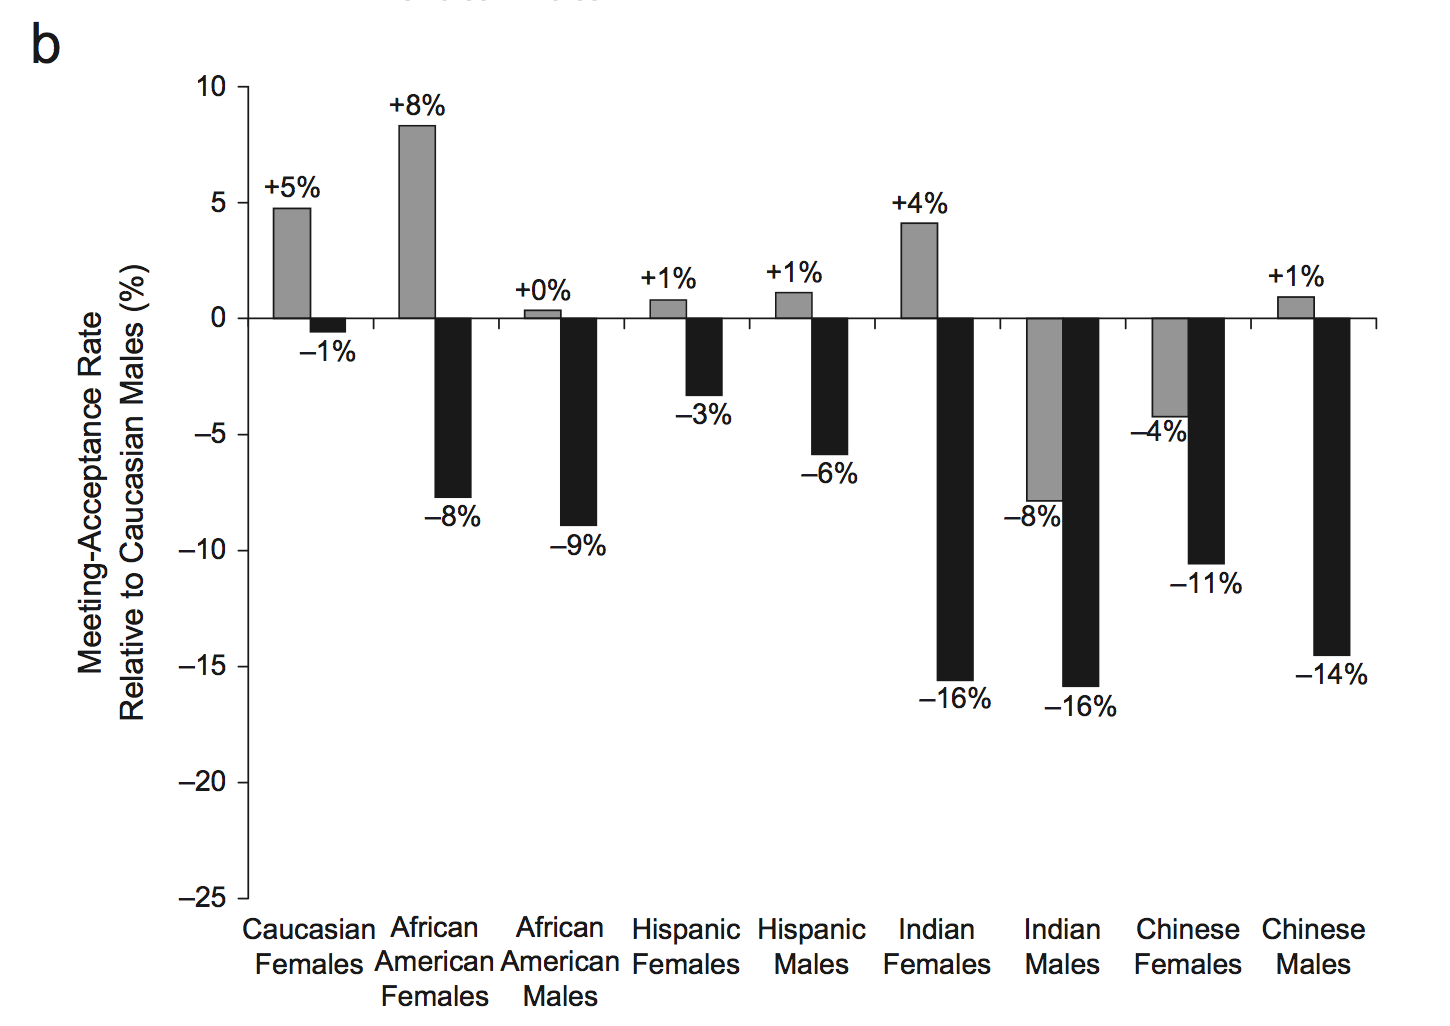
\includegraphics[width=0.8\textwidth]{figures/milkman_temporal_2012_fig2b.png}
\end{figure}

\end{frame}
%%%%%%%%%%%%%%%%%%%%%%%%
\begin{frame}

What are the fixed and variable costs for this experiment?

\end{frame}
%%%%%%%%%%%%%%%%%%%%%%%%
\begin{frame}

{\Large
\begin{center}
Important difference between:\\
zero variable cost and zero variable cost to you
\end{center}
}

\end{frame}
%%%%%%%%%%%%%%%%%%%%%%%%
\begin{frame}

\begin{center}
\Large Questions?
\end{center}

\end{frame}
%%%%%%%%%%%%%%%%%%%%%%%%


\end{document}
